\chapter{Background}\label{cap:estadodelarte}

\noindent This second chapter tries to acquaint the reader with the key concepts that define Cloud Computing as well as the MapReduce archetype. Later successive elaborations to the project will lay on top of them.

\section{Cloud Computing}\label{sec:computacioncloud}

\noindent In essence, Cloud Computing, or Cloud for short, is a distributed computing model that attempts to ease the consumption on-demand of that distributed infrastructure, by exporting it as virtual computational resources, platforms or services. However it may seem, the Cloud is no new technology but it introduces a new manner to exploit idle computing capacity. What it intends is to make orchestration of enormous data centers more flexible, so as to allow a user to start or destroy virtual machines as required --- Infrastructure as a Service (\emph{IaaS}) ---, leverage a testing environment over a particular Operating System or software platform --- Platform as a Service (\emph{PaaS}) --- or use a specific service like remote backup --- Software as a Service (\emph{SaaS}). Figure \ref{fig:cloudlayers} shows the corresponding high level layer diagram of a generic Cloud.

\begin{figure}[tbp]
\begin{center}
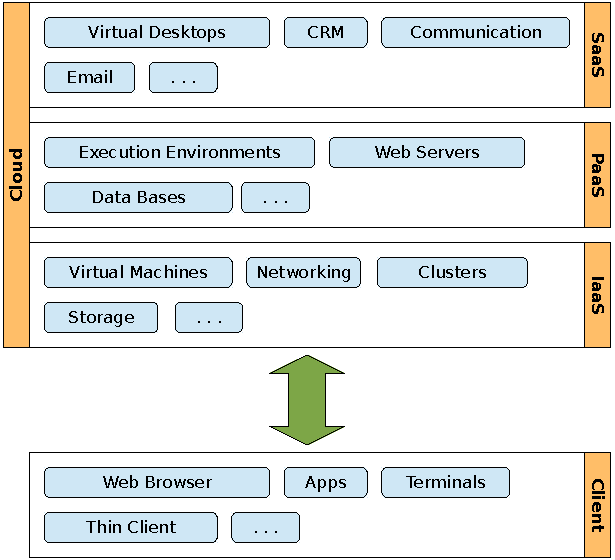
\includegraphics[width=0.69\textwidth]{imagenes/003.pdf}
 \caption{Layers in a cloud in production}
\label{fig:cloudlayers}
\end{center}
\end{figure}

Different IaaS frameworks will cover the functionality that is required to drive the cloud-defining \emph{physical} infrastructure. Nonetheless, an effort to analyze, design, configure, install and maintain the intended service will be needed, bearing in mind that the degree of elaboration grows from IaaS services to SaaS ones. In effect, PaaS and SaaS layers are lied supported by those immediately under --- software is implemented over a particular platform which, in turn, is also build upon a physical layer. Every Cloud Framework focuses on giving the option to configure a stable environment in which to run virtual machines defined by four variables: Virtual CPU count, virtual RAM, virtual persistent memory and virtual networking devices. Such an environment makes it possible to deploy virtual clusters upon which to install platforms or services to be subsequently consumed by users, bringing up the software layers that give form PaaS and SaaS paradigms respectively.

No less important cuestions like access control, execution permissions, quota or persistent or safe storage will also be present in all of the frameworks.


\subsection{Architecture}\label{subsec:arquitecturacloud}

\noindent Figure \ref{fig:cloudlayers} showed possible layers that could be found in a cloud deployment. Depending on the layers that are implemented, the particular framework and the role played by the cluster node, different particular modules will appear to make possible the consumption of configured services. These modules may be though of as Cloud subsystems that connect each one of the parts that are required to execute virtual machines. Those virtual machines' capabilities are defined by the four variables previously discussed --- VCPUS, RAM, HDD and networking. As there is no methodology dictating how those subsystems should be in terms of size and responsibility, and thus, each framework makes its own modular partition regarding infrastructure management.

Setting modularity apart, one common feature among different clouds is the separation of responsibility in two main roles: \emph{Cloud Controller} and \emph{Cloud Node}. Figure \ref{fig:archcloud} shows a generic Cloud deployment in a cluster with both roles defined. The guidelines followed for having this two roles lies close to \emph{Master-Slave} architectures' approach. In those, in the abstract, there's a set of computers labeled as coordinators which are expected to control execution, and another set made up with those machines that are to carry out the actual processing.

\begin{figure}[tbp]
\begin{center}
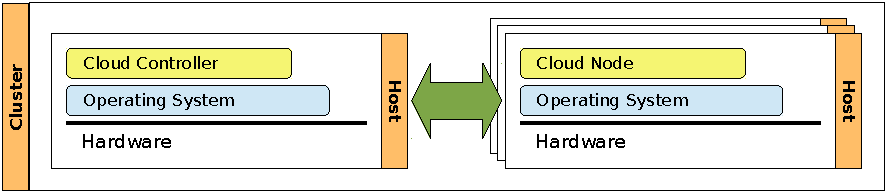
\includegraphics[width=0.9\textwidth]{imagenes/004.pdf}
 \caption{Cloud Controller and Cloud Node}
\label{fig:archcloud}
\end{center}
\end{figure}

Within this general role distribution in a cluster, host computers or cluster nodes --- labeled as Cloud Controllers or Cloud Nodes --- cooperate in a synchronized fashion through \emph{NTP} (\emph{Network Time Protocol}) and communicate via message passing supported by asynchronous queues. To store services' metadata and status they typically draw upon a \emph{DBMS} (\emph{Data Base Management System}) implementation, which is regularly kept running in a dedicated cluster node set sharded (distributed) between the members of the set.

Although there is no practical restriction to configuring both Cloud Controller and Cloud Node within a single computer in a cluster, this approach should be limited to development environments due to the considerable impact in performance that it would carry.


\subsubsection{Cloud Controller}\label{subsubsec:cloudcontroller}

\noindent The fundamental task for a Controller is to maintain all of the cloud's constituent modules working together by coordinating their cooperation. As an example, it is a Controller's duty to:

\begin{itemize}
 \item Authentication and authorization control.
 \item Available infrastructure resources recount.
 \item Quota management.
 \item Usage balance.
 \item User and project inventory.
 \item API exposure for service consumption.
 \item Real time cloud monitoring.
\end{itemize}

Being an essential part of a cloud as it is, the Controller node (not to be mistaken for the Cloud Node) is usually replicated in physically distinct computers. Figure \ref{fig:cloudcontroller} shows a Cloud Controller's architecture from a high level perspective.

\begin{figure}[tbp]
\begin{center}
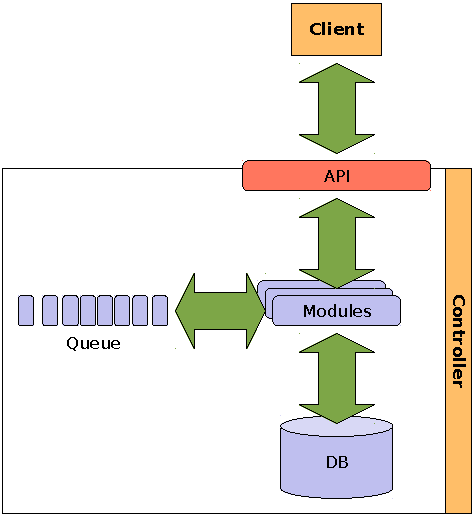
\includegraphics[width=0.5\textwidth]{imagenes/005.pdf}
 \caption{Cloud Controller in detail}
\label{fig:cloudcontroller}
\end{center}
\end{figure}

As a general rule, clients will interact with clouds through a Web Service API --- mostly \emph{RESTful} APIs (\emph{REpresentational State Transfer}). Those APIs vary slightly from company to vendor as usual, which forces clients to be partially coupled to clouds. That is why there has been an increasing trend for unifying and standardizing those APIs in order to guarantee compatibility inter-framework. Of special mention is the cloud standard proposed by the \emph{Open Grid Forum}: \emph{OCCI} (\emph{Open Cloud Computing Interface} \cite{occisdraft}).

The cloud's conforming modules support its functional requirements. Each one of them will have a well-defined responsibility, and so appear networking modules, access and security control modules, storage modules, etc. Many of them existed before the advent of Cloud Computing but they worked only locally. Inter-module communication is handled by means of an asynchronous message queue that guarantees an equally efficient broadcasting system outside of the Cloud Controller, i.e. the rest of the cluster nodes participating in the cloud.

To store and expose configuration data to the cluster in a single place while managing concurrent requests to update these data, every IaaS Framework evaluated resorts to a DBMS whose profiling must be properly tailored.

Hardware requirements on the cluster nodes vary from each particular framework implementation and the \emph{QoS} expected, but, in the abstract, they normally need something around 10 GB of RAM, quad core CPU, Gigabit Ethernet and one TB of storage.


\subsubsection{Cloud Node}\label{subsubsec:cloudnode}

\noindent If the Cloud Controller is entrusted the cloud's correct functioning acting like a glue for its parts, the actual task processing is performed in the Cloud Nodes; that is, the VCPU, VRAM, VHDD are going to be mapped from the corresponding CPU, RAM and HDD from the real nodes of the cluster.

Cloud Nodes may be heterogeneous according to their hardware characteristics. They will configure a resource set that, seen from the outside of the cluster, will appear to be a homogeneous whole where the summation of capacities of every participating node is the cloud's dimension. Further, this homogeneous space could be provisioned, as discussed above, on demand. It is the Cloud Controller's responsibility single out the optimal distribution of virtual servers throughout the cluster, attending to the physical aspects of both the virtual machine and the computer in which the former will run.

The most important subsystem in a Cloud Controller is the \emph{hypervisor} or \emph{VMM} (\emph{Virtual Machine Monitor}). The hypervisor is responsible for making possible the execution of virtual servers --- or virtual instances following the AWS nomenclature --- by creating the virtual architecture needed and a \emph{virtual execution domain} managed with the help of the operating system kernel. To generate this architecture there fundamentally exist three techniques: \emph{Emulation}, \emph{Paravirtualization} and \emph{Hardware Virtualization} or \emph{Full Virtualization}. Different hypervisors will support them in a different degree, but most will cover only one of them.

\subsection{Virtualization Techniques}\label{subsec:tecnicasemu}

\noindent What follows is a brief review of the main methods to create virtual infrastructure.

\subsubsection{Emulation}\label{subsubsec:emulacion}

\noindent Emulation is the most general virtualization method, in a sense that it does not call for anything special be present in the underlying hardware. However, it also carries the highest penalization in terms of performance. With emulation, every structure sustaining the virtual machine operation is created as a functional software copy of its hardware counterpart; i. e., every machine instruction to be executed in the virtual hardware must be run software-wise first, and then be translated on the fly into another machine instruction runnable in the physical domain --- the cluster node. The interpreter implementation and the divergence between emulated and real hardware will directly impact the translation overhead. This fact hinders the emulation from being widely employed in performance-critical deployments. Nonetheless, thanks to its operating flexibility it's generally used as a mechanism to support legacy systems. Besides, the kernel in the guest operating system --- the kernel in the virtual machines's --- operating system needs no alteration whatsoever, and the cluster node's kernel need only load a module.

\subsubsection{Hardware Virtualization}\label{subsubsec:virthardware}

\noindent Hardware Virtualization, on the contrary, allows host's processes to run directly atop the physical hardware layer, with no interpretation. Logically, this provides a considerable speedup from emulation, though imposes a special treatment to be given to its virtual processes. Regarding CPUs, both AMD's and Intel's support virtual process execution --- which is the capacity to run processes belonging to the virtual domain with little performance overhead --- as far as the convenient hardware extensions are present (\emph{SVM} and \emph{VT-x} respectively \cite{intelvtx}). Just as what happened with emulation, an unaltered host's kernel may be used. This fact is of relative importance as if wasn't so it would limit the myriad of OSs that could be installed as guests. Lastly, it should be pointed out that the hardware architecture is exposed to the VM as it is, i. e. with no software middleware.

\subsubsection{Paravirtualization}\label{subsubsec:paravirt}

\noindent Paravirtualization uses a different approach. To begin with, it is indispensable that the guest's kernel be modified to make it capable of interacting with a paravirtualized environment. When the guest runs, the hypervisor will separate those regions of instructions that have to be executed in kernel mode in the CPU, from those in user mode which will be executed as regular host processes. Subsequently, the hypervisor will manage an on-contract execution between host and guest allowing the latter to run kernel mode sections as if pertaining to the real execution domain --- as if they were processes running in the host, not in the guest --- with almost no performance slowdown. Paravirtualization, in turn, does not require an special hardware extension be present.

\subsection{Cloud IaaS frameworks}\label{subsec:frameworksiaas}

\noindent Cloud IaaS frameworks are those software systems managing the abstraction of complexity associated with on demand provisioning and administering failure-prone generic infrastructure. In spite of being almost all of them open sourced --- which fosters reusability and collaboration ---, they have evolved in different frames. This fact has raised a condition of lacking outwards interoperability, maturing non-standard APIs; though today those divergences are fading away. These frameworks and APIs are product of the efforts to improve and ease controlling the underlying particular clusters on which they germinated. Thus, it is no surprising their advances had originated parallelly with the infrastructure they drove, leaving compatibility in the background.

Slowly but steadily these managing systems became larger in reach and responsibility boosted by an increasingly interest in the sector. In the end, it happened that software and systems engineering made them more abstract, so they finally overlapped functionally. AWS appearance finished forging the latent standardization need, and thus, as of today, most frameworks offer APIs closer and closer to Amazon's --- nowadays the de-facto standard --- and OCCI's \cite{occisdraft}.

\section{MapReduce Paradigm}\label{sec:mapred}

\noindent The origin of the paradigm centers around a paper publication of two Google employees \cite{googlemapreduce}. In this paper they explained a method implementation devised to abstract the common parts present in distributed computing that rendered simple but large problems much more complex to solve when paralleling their execution on massive clusters. A concise definition states that MapReduce is ``\textit{a data processing model and execution environment that runs on large clusters of commodity computers}'' \cite{hadoopdefguide}.

\subsection{Programming Model}\label{subsec:programacionmapred}

\noindent The MapReduce programming model requires the developer express his problem as a partition of two well-defined pieces. A first part deals with the reading of input data and with producing a set of intermediate results that will be scattered over the cluster nodes. These intermediate transformations will be grouped according to an intermediate key value. A second phase begins with that grouping of intermediate results and concludes when every \emph{reduce} operation on the groupings succeeds. Seen from another vantage point, the first phase corresponds, broadly speaking, to the behavior of the functional \emph{map} and the second to the functional \emph{fold}.

In terms of the MapReduce model, these functional paradigm concepts give rise to \emph{Map} and \emph{Reduce} functions. Both Map and Reduce have to be supplied by the developer, which may force a deviation in breaking the original problem down. As counterpart, the MapReduce model will deal with parallelizing the computation, distributing input data across the cluster, handling exceptions that could raise and recovering output results; everything transparent to the programmer.

\subsubsection{Funci\'on Map}\label{map}

\noindent The typical functional map takes any function \emph{F} and a list of elements \emph{L} or, in general, any recursive data structure, to return a list resulting from applying \emph{F} to each element of \emph{L}. Figure \ref{fig:functionalmap} shows its signature and an example.

\begin{figure}[tbp]
\begin{center}
\begin{tabular}{|l|}
\hline
$\mathbf{map:} \: \left ( \alpha \rightarrow \beta \right ) \: \rightarrow \: \alpha \: list \: \rightarrow \: \beta \: list$ \\
$\mathbf{map} \: \left( \mathbf{pow}\:2 \right) \: \left[ 1,2,3 \right] \: \Rightarrow \: \left[ 1,4,9 \right ]$ \\
\hline
\end{tabular}
\caption{Map function example (functional version)}
\label{fig:functionalmap}
\end{center}
\end{figure}

In its MapReduce realization, map function receives a tuple as input and produces another tuple \emph{(key, value)} as intermediate output. It is the MapReduce library who is responsible for feeding the map function by mutating the data contained in input files into \emph{(key, value)} pairs. Then, it deals with grouping those intermediate tuples by key before passing them in as input to the reduce function. Input and output data types correspond to those shown in the function signature figure \ref{fig:mapreducemap}.

\begin{figure}[tbp]
\begin{center}
\begin{tabular}{|l|}
\hline
$\mathbf{map:} \: \left( k1,v1 \right) \: \rightarrow \: \left( k2,v2 \right) list$ \\
$\mathbf{k:} \: clave \linebreak$ \\
$\mathbf{v:} \: valor \linebreak$ \\
$\mathbf{\left(kn,vn \right):} \: par \: \left( clave,valor \right) \: en \: un \: dominio \: n$ \\
\hline
\end{tabular}
\caption{Map function signature (MapReduce version)}
\label{fig:mapreducemap}
\end{center}
\end{figure}


\subsubsection{Reduce function}\label{reduce}

\noindent The typical functional fold expects any function \emph{G}, a list \emph{L}, or generally any type of recursive data structure, and any initial element \emph{I}, subtype of \emph{L}'s elements. Fold returns the value in \emph{I} resulting from building up the intermediate values generated after applying \emph{G} to each element in \emph{L}. Figure \ref{fig:fold} presents fold signature as well as an example.

\begin{figure}[tbp]
\begin{center}
\begin{tabular}{|l|}
\hline
$\mathbf{fold:} \: \left( \alpha \rightarrow \beta \rightarrow \alpha \right) \: \rightarrow \: \alpha \: \rightarrow \: \beta \: list \: \rightarrow \: \alpha$ \\
$\mathbf{fold} \: \left( \mathbf{+} \right) \: 0 \: \left[ 1,2,3 \right] \: \Rightarrow \: 6$ \\
\hline
\end{tabular}
\caption{Fold function example}
\label{fig:fold}
\end{center}
\end{figure}

Contrary to map, reduce expects the intermediate groups as input to produce a smaller set of values for each group as output, because reduce will iteratively \emph{fold} the groupings into values. Those reduced intermediate values will be passed in again to the reduce function if more values with the same key appeared from subsequent maps. Reduce signature is shown on figure \ref{fig:reduce}. Just as happens with map, MapReduce handles the transmission of intermediate results out from map into reduce. The model also describes the possibility to define a \emph{Combiner} function that would act after map partially reducing the values within the same grouping to lower network traffic --- the combiner usually runs in the same machine as the map.

\begin{figure}[tbp]
\begin{center}
\begin{tabular}{|l|}
\hline
$\mathbf{reduce:} \: \left( k2,v2 \: list \right) \: \rightarrow \: v2 \: list$ \\
$\mathbf{k:} \: clave$ \\
$\mathbf{v:} \: valor$ \\
$\mathbf{\left(kn,vn \right):} \: par \: \left(clave,valor\right) \: en \: un \: dominio \: n$ \\
\hline
\end{tabular}
\caption{Reduce function signature}
\label{fig:reduce}
\end{center}
\end{figure}

\subsubsection{A word counter in MapReduce}\label{subsubsec:wordcount}

\noindent As an example, figure \ref{fig:wordcount} shows the pseudocode of a MapReduce application to count the number of words in a document set.

\begin{figure}[tbp]
 \begin{center}
  \begin{tabular}{|l|}
   \hline
   \texttt{{\bf Map} (String key, String value):} \\
   \texttt{// key: documento name} \\
   \texttt{// value: document contents} \\
   \texttt{{\bf for each} word w {\bf in} value:} \\
   \texttt{{\bf EmitIntermediate} (w, ``1'')};\\ \\

   \texttt{{\bf Reduce} (String key, Iterator values):} \\
   \texttt{// key: a word} \\
   \texttt{// values: an Iterable over intermediate counts of the word key} \\
   \texttt{{\bf int} result = 0;} \\
   \texttt{{\bf for each} v {\bf in} values:} \\
   \texttt{{\bf Emit} ({\bf AsString} (result));} \\
   \hline
  \end{tabular}
  \caption{MapReduce wordcount pseudocode. Source: \cite{googlemapreduce}}
  \label{fig:wordcount}
 \end{center}
\end{figure}

In a wordcount execution flow the following is going to happen: map is going to be presented with a set of names containing all of the documents in plain text whose words will be counted. Map will subsequently iterate over each document in the set emitting the tuple \emph{(<word>, ``1'')} for each word found. Thus, an explosion of intermediate pairs will be generated as output of map, will be distributed over the network and progressively folded in the reduce phase. Reduce is going to be input every pair generated by map but under a different form. Reduce will accept on each invocation the pair \emph{(<word>, list(``1''))}. The list of \emph{``1''}s, or generically an \texttt{Iterable} over \emph{``1''}s, will contain as many elements as instances of the word \emph{<word>} there were in the document set --- this supposing that the map phase were over before starting the reduce phase and that every word \emph{<word>} were submitted to the same reducer in the cluster --- a cluster node executing the reduce function.

Once the flow had been completed, MapReduce would return a listing with every word in the documents and the number of times it appeared.

\subsection{Applicability of the Model}\label{subsec:aplicabilidad}

\noindent The myriad of problems that could be expressed following the MapReduce programming parading is clearly reflected in \cite{googlemapreduce}, a subset of them being:

\begin{itemize}
 \item Distributed grep: Map emits every line matching the regular expression. Reduce only forwards its input to its output acting as identity function.
 \item Count of URL access frequency: Like wordcount.
 \item Reverse web-link graph: For each URL contained in a web document, map generates the pair \emph{(<target\_URL>, <source\_URL>)}. Reduce will emit the pair \emph{(target, list(source))}.
 \item Inverted index: Map parses each document and emits a series of tuples in the form \emph{(<word>, <document\_id>)}. All of them are passed as input to reduce that generates the sequence of pairs \emph{(<word>, list(document\_id))}.
\end{itemize}

\subsection{Processing Model}\label{subsec:processingmodel}

\noindent Besides defining the structure that the applications willing to leverage the MapReduce capabilities will have to follow --- so that they need not code their own distribution mechanisms ---, with \cite{googlemapreduce} an implementation of the model was introduced which allowed Google to stay protocol, architecture and system agnostic while keeping their commodity clusters on full utilization. This agnosticism allows for deploying vendor-lock-free distributed systems.

The MapReduce model works by receiving self-contained processing requests called \emph{job}s. Each job is a \emph{partition} of smaller duties called \emph{task}s. A job won't be completed until no task is pending for finishing execution. The processing model main intent is to distribute the tasks throughout the cluster in a way that reduced job latency. In general, it can be stated that task processing on each phase is done in parallel and phases execute in sequence; yet, it is not needed for reduce to wait until map is complete.

Figure \ref{fig:exmapreduce} shows a summary of a typical execution flow. It is interesting enough to deepen in its details as many other MapReduce implementations will present similar approaches.

\begin{figure}[tbp]
\begin{center}
 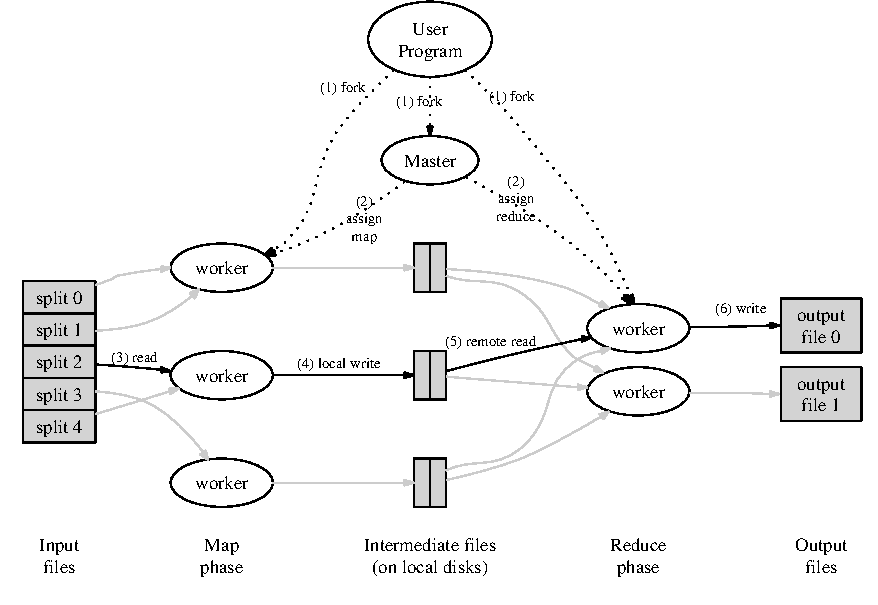
\includegraphics[width=0.9\textwidth]{imagenes/006.pdf}
 \caption{MapReduce execution diagram. Source: \cite{googlemapreduce}}
 \label{fig:exmapreduce}
\end{center}
\end{figure}

\begin{enumerate}
 \item MapReduce divides input files in \emph{M} parts, the size of which is parameterized, and distributes as many copies of the MapReduce user algorithm as nodes participate in the computation.
 \item From this moment each program copy resides in a cluster node. A random copy is chosen among them and labeled as the \emph{Master Replica}, effectively assigning the \emph{Master Role} to the node holding the replica; every other node in the cluster is designated with the \emph{Worker Role}. Those worker nodes will receive the actual MapReduce tasks and their execution will be driven from the master node. There will be \emph{M} map tasks and \emph{R} reduce tasks.
 \item Workers assigned with map tasks read their corresponding portions of the input files and parse the contents generating tuples \emph{(key, value)} that will be submitted to the map function for processing. Map outputs are stored in memory as a cache.
 \item Periodically, those pairs in memory are dumped to a local disk --- dumped to a drive of the node that is executing the map function --- and partitioned into \emph{R} regions. Their path on disk is then sent back to the master, responsible for forwarding these paths to \emph{reduce workers} or \emph{reducer}s.
 \item Now, when a reducer is notified that it should start processing, the path to the data of the reduction is send along and the reducer will fetch them directly from the mapper via \emph{RPC} (\emph{Remote Procedure Call}). Before actually invoking the reduce function, the node itself will sort the intermediate pairs by key.
 \item Lastly, the reducer iterates over the key-sorted pairs submitting to the user-defined reduce function the key and the \texttt{Iterable} of values associated to the key. The output fo the reduce function for the reducer partition is appended to a file stored over the distributed file system.
\end{enumerate}

When every map and reduce tasks had succeeded, the partitioned output space --- the file set within each partition --- would be returned back to the client application that had made the MapReduce invocation.

This processing model is abstract enough as to be employed to the resolution of indeterminatedly large problems running on huge clusters.

\subsection{Fault Tolerance}\label{subsec:toleranciafallos}

\noindent The idea of providing an environment to execute jobs long enough to require large sets of computing machines to keep the latency within reasonable timings, calls for the definition of a policy able to assure a degree of tolerance to failure. If unattended, those failures would lead to errors; some would cause finished tasks to get lost, others would put intermediate data offline. Consequently, if no measures were taken to prevent or deal with failure, job throughput would humble as some would have to be rescheduled all along.

The MapReduce model describes a policy foreseeing a series within an execution flow and duly implements a series of actions against them.

\subsubsection{Worker Failure}\label{subsubsec:fallotrabajador}

\noindent The least taxing of the problems. To control that every worker is up, the master node pings them periodically. If a worker did not reply to pings repeatedly, it would be marked as failed.

A worker marked failed will neither be scheduled new tasks nor will be remotely accessed by reducers to load intermediate map results that it may had; a fact that could prevent the workflow from succeeding. If so were the case, the access to these data would be resolved by the master labeling the results of the failing tasks as \emph{idle}, so that they could be rescheduled a later time to store the results in an active worker.

\subsubsection{Master Failure}\label{subsubsec:fallomaestro}

Failure of a master node is more troublesome. The proposed approach consists in making the master periodically create a snapshot from which to restore to a previous state if it went unexpectedly down. It is a harder problem than a worker failure mainly because there can only be one master per cluster, and the time it would take another node to take over the master role would leave the scheduling pipeline stalled. The master being in a single machine has also the benefit of lowering the probability of failure, precisely why in the original paper \cite{googlemapreduce} it had been put forward that the entire job be canceled. Still, as there is no good design to leave a \emph{single point of failure}, subsequent MapReduce implementations have proposed to replicate the master in other nodes in the same cluster.

\subsection{Aditional Characteristics}\label{subsec:caracteristicasadicionales}

\noindent What follows is a summary of additional features of the original MapReduce implementation.

\subsubsection{Locality}\label{subsubsec:localidad}

\noindent The typical bottleneck in a modern deployment is network bandwidth. In MapReduce executions, the information flows into the cluster from the external client. As already discussed, each node in a MapReduce cluster holds a certain amount of the input data and shares its processing capacity to be used for particular MapReduce tasks over those data. Each stage in the MapReduce executing pipeline requires a lot of traffic to be handled by the network which would reduce throughput if no wide enough channel were deployed nor a locality exploiting strategy were implemented.

In fact, MapReduce explores a method to use locality as an additional resource. The idea is for the distributed file system to place data as close as possible to where they will transformed --- it will try to store data in the mappers' and reducers' local drives ---, effectively diminishing the transport over the net.

\subsubsection{Complexity}\label{subsubsec:complejidad}

\noindent A priori, variables \emph{M} and \emph{R}, the number of partitions of the input space and of the intermediate space respectively, may be configured to take any value whatsoever. Yet, there exist certain practical limits to their values. For every running job the master will have to make $O(M + R)$ scheduling decisions --- if no error forced the master to reschedule tasks ---, as each partition of the input space will have to be submitted to a mapper and each intermediate partition will have to be transmitted to a reducer, coming to $O(M + R)$ as the expression of \emph{temporal complexity}. Regarding \emph{spatial complexity}, the master will have to maintain $O(M \cdot R)$ as piece of state in memory as the intermediate results of a map task may be propagated to every piece \emph{R} of the reduce space.

\subsubsection{Backup Tasks}\label{subsubsec:secundarias}

\noindent A situation could arise in which a cluster node be executing map or reduce tasks much slower than it theoretically could. Such a circumstance may arise with a damaged drive which would cause read and write operations to slow down. And since jobs complete when all of its composing tasks had been finished, the faulted node (\emph{the straggler}) would be curbing the global throughput. To alleviate this handicap, when few tasks are left incomplete for a particular job, \emph{Backup Task}s are created an submitted to additional workers, making a single task be executed twice concurrently. By the time one copy of the task succeeds it will be labeled completed, duly reducing the impact of stragglers at the cost of wasting computational resources.

\subsubsection{Combiner Function}\label{subsubsec:combiner}

\noindent Many times it happens that there exists a good number of repeated intermediate pairs. Taking wordcount as an example, it can be easily seen that every mapper will generate as many tuples \emph{(``a'', ``1'')} as \emph{a}'s there are in the input documents. A mechanism to lower the tuples that will have to be emitted to reducers is to allow for the definition of a \emph{Combiner Function} to group outputs from the map function --- and in the same mapper node --- before sending them out over the network, effectively cutting down traffic.

In fact, it is usual for both combiner and reduce functions to share the same implementation, even though the former writes its output to local disk while the latter writes directly to the distributed file system.

\subsection{Other MapReduce Implementations}\label{subsec:frameworksmapred}

\noindent Since 2004 multiple frameworks that implement the ideas exposed in the paper \cite{googlemapreduce} have been coming out. The next listing clearly shows the impact MapReduce has created.

\begin{description}
 \item[Hadoop] \cite{hadoopdefguide} One of the first implementations to cover the MapReduce processing model and framework of reference to other MapReduce codifications. It is by far the most widely deployed, tested, configured and profiled today.
 \item[GridGain] \cite{gridgainvshadoop} Commercial and centered around in-memory processing to speedup execution: lower data access latency at the expense of smaller I/O space.
 \item[Twister] \cite{twister} Developed as a research project of the University of Indiana, tries to cut out and abstract the common parts required to run MapReduce workflows in order to keep them longer in the cluster's distributed memory. With such an approach, the time taken to configure mappers and reducers in multiple executions is lowered by doing the set up only once. Thus, \emph{Twister} really shines in executing \emph{iterative} MapRecude jobs --- those jobs where maps and reduces do not happen in sequence once, but need instead a multitude of complete map-reduce cycles to succeed.
 \item[GATK] \cite{gatk} Used for genetic research to sequence and evaluate DNA fragments from multiple species.
 \item[Qizmt] \cite{qizmt} Written in C\# and deployed in MySpace.
 \item[misco] \cite{misco} Written 100\% Python and based on previous work at Nokia it is posed as a MapReduce implementation capable of running in mobile devices.
 \item[Peregrine] \cite{peregrine} By optimizing how intermediate results are transformed and by passing every I/O operation throughout an asynchronous queue, its developers claim to have formidably accelerated task execution rate.
 \item[Mars] \cite{mars} Implemented in \emph{NVIDIA CUDA}, it revolves around extracting higher performance by moving the map and reduce operations into the graphic card. It is supposed to improve processing throughput by over an order of magnitude.
\end{description}

Hadoop is undoubtedly the MapReduce implementation more used nowadays. Its open source nature and its flexibility, both for processing and storing, have constantly reported back an increasing interest from the IT industry. This has brought out many pluggable extensions that enhance Hadoop's applicability. 
